\documentclass[dvipdfmx]{beamer}
\usetheme[secheader]{Boadilla}
% \usepackage{beamerthemesplit} // Activate for custom appearanced
%\setbeamertemplate{caption}[numbered]
\usefonttheme[onlymath]{serif} %数式をゴシックにしない
\setbeamertemplate{blocks}[rounded] % Blockの影を消す
\useinnertheme{circles} % 箇条書きをシンプルに
\setbeamertemplate{navigation symbols}{} % ナビゲーションシンボルを消す
\setbeamertemplate{footline}[frame number] % フッターはスライド番号のみ
\setbeamercolor{page number in head/foot}{fg=black}
% \usepackage{beamerthemesplit} // Activate for custom appearance
\setlength{\parindent}{1em}  %段落字下げ
\renewcommand{\figurename}{Fig}
\renewcommand{\tablename}{Tab}
\usepackage{tikz}  
\usetikzlibrary{decorations.pathreplacing,calligraphy}
\setbeamerfont{itemize/enumerate subbody}{size=\normalsize}
%\setbeamertemplate{itemize subitem}{\normalsize\raise1.25pt\hbox{\donotcoloroutermaths$\blacktriangleright$}}  %to set the symbol size


\title{非負値行列因子分解の統一的な拡張と医学データ解析}
\date{2023年6月3日}
\author {阿部興\footnote{名古屋大学医学系研究科} ・ 島村徹平\footnote{名古屋大学医学系研究科・東京医科歯科大学難治疾患研究所}}

\begin{document}
\frame{
\titlepage
}

\renewcommand*{\thefootnote}{\fnsymbol{footnote}}
\setcounter{footnote}{0} 

\section{背景}
\frame{
\frametitle{背景}

\begin{itemize}
\item 生命科学に関わる多数の要素の縦断的な観測が可能に
\begin{itemize}
\item ゲノム, エピゲノム, トランスクリプトーム, プロテオーム, ...
\end{itemize}
\item これらは非負の整数(カウント)データ
\item 計算機上では多次元配列(テンソル)
\item 欠損や重複の扱いが難しい
\end{itemize}
}
\frame{
\frametitle{tidy data}

\begin{figure}
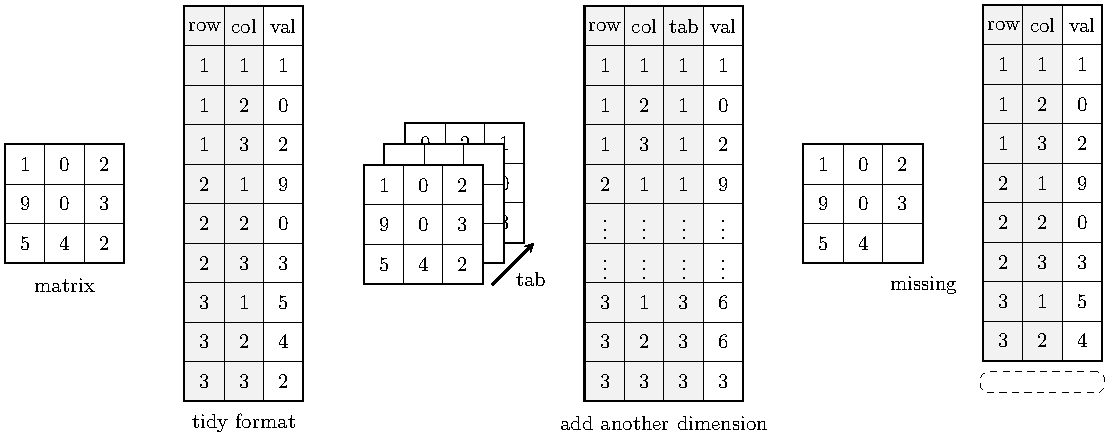
\includegraphics[width=10cm]{./img/tidy_concept.pdf}
\end{figure}
\begin{itemize}
     \item 各変数が 1 つの列を形成する
     \item 各観測値が 1 つの行を形成する
     %\item 各観測の観測単位の種類が 1 つのテーブルを形成する
     \item 各値が 1 つのセルを構成する
\end{itemize}
}
\frame{
\begin{figure}
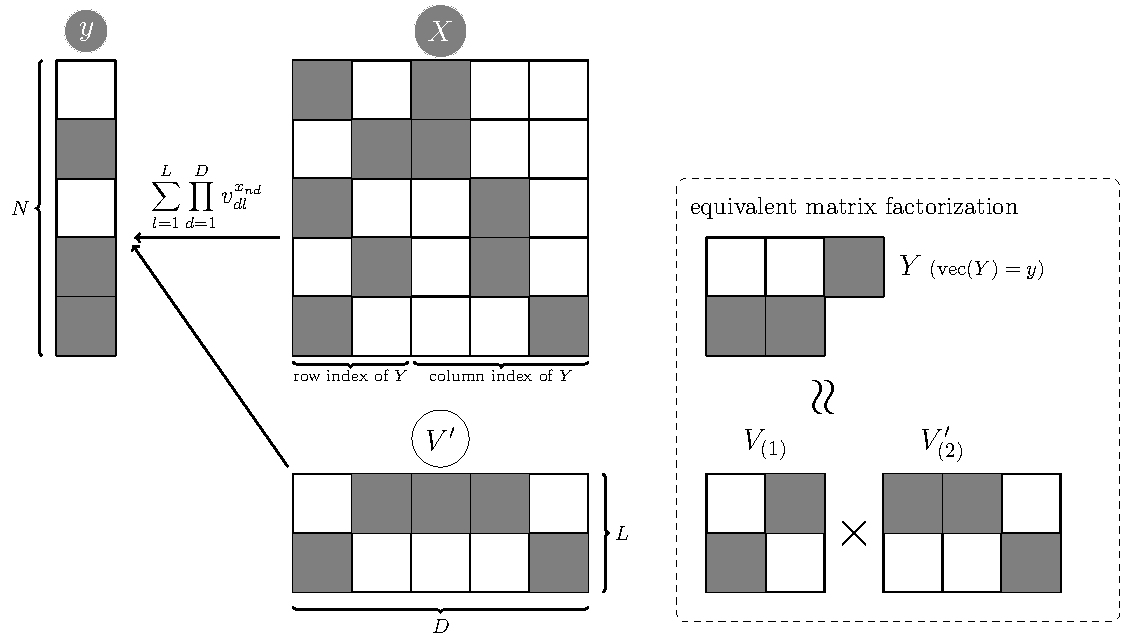
\includegraphics[width=10.5cm]{./img/product.pdf}
\caption{UNMFのコンセプト. 灰色:観測される変数,  白:潜在変数(推定の対象)}
\end{figure}
%\footnote{Abe K \& Shimamura T. (2023). UNMF: A unified non-negative matrix factorization for multi-dimensional omics data. {\em Briefings in Bioinformatics.} (Under Review)}
}
\frame{

\begin{figure}
$y_{n}  \approx \sum_{l}\prod_{d}v_{dl}^{x_{nd}}$\\
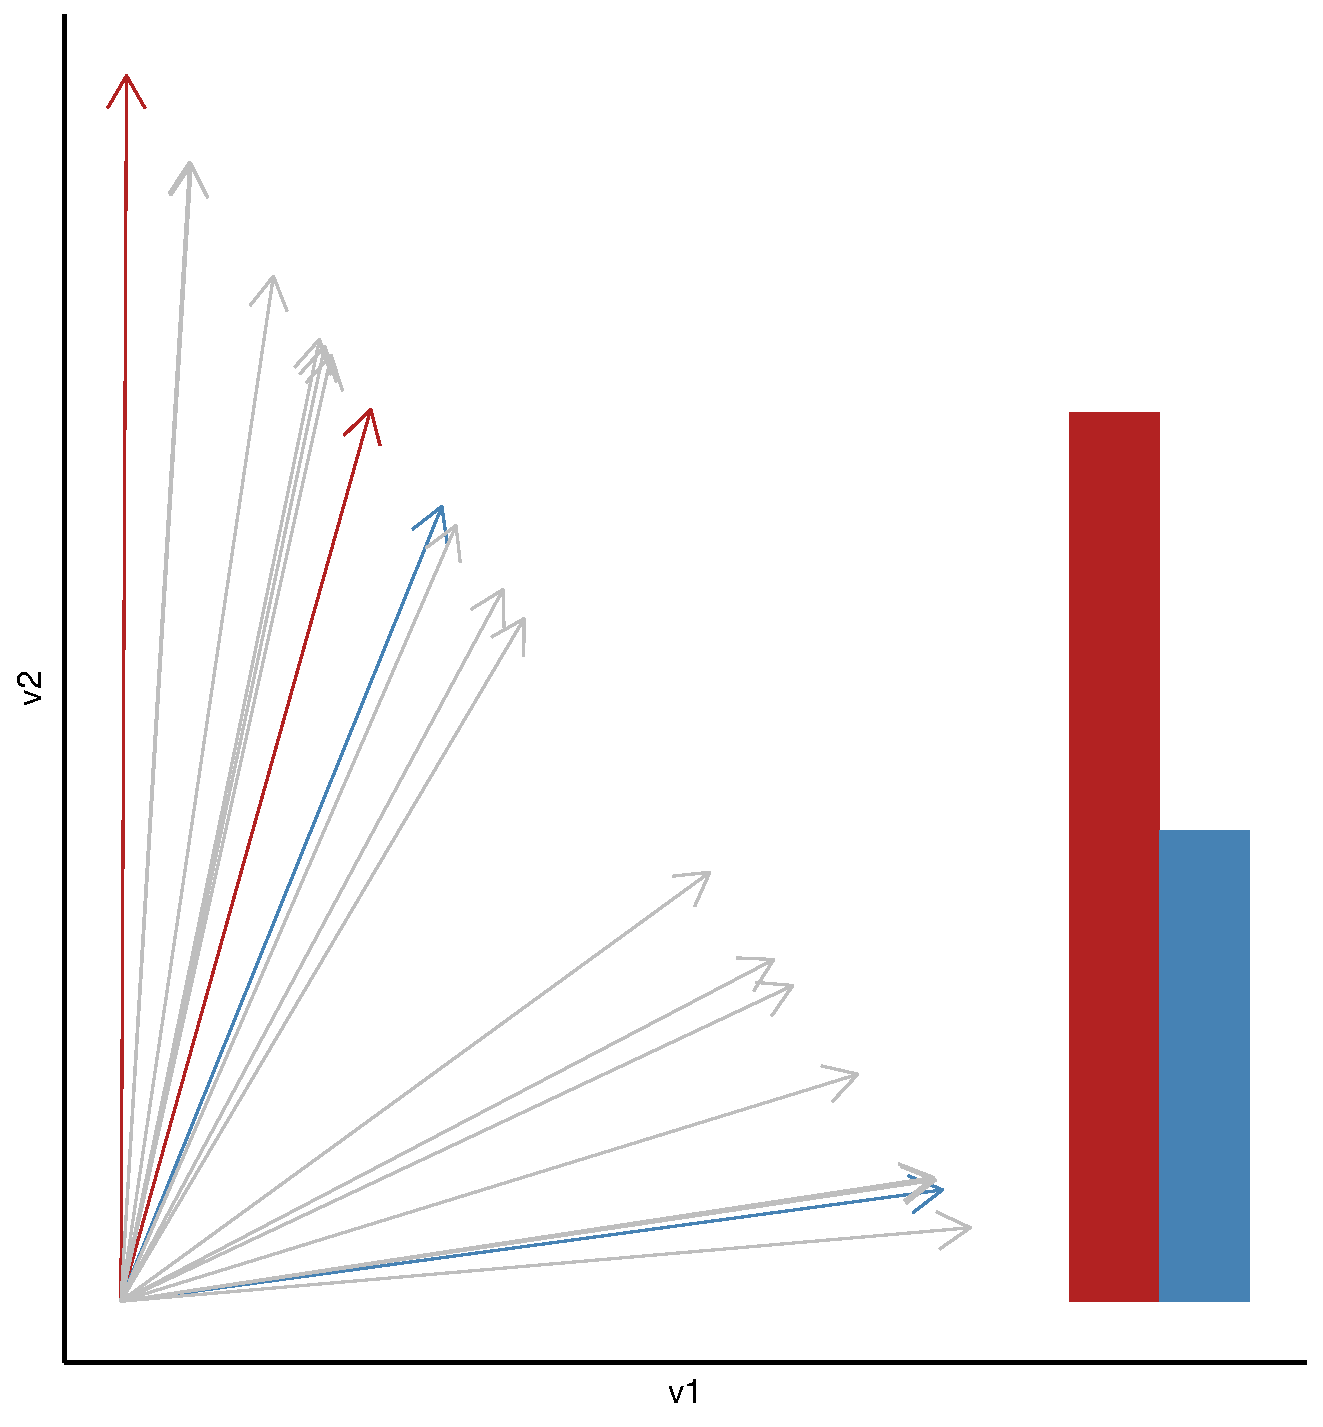
\includegraphics[width=5.5cm]{./img/mprod.pdf}
\caption{$x$で指定されるベクトルどうしの向きが近いほど右辺が大きくなる}
\end{figure}
}
\section{モデルと推定}
\frame{
\frametitle{表記法}

\begin{itemize}
\item 確率分布(密度関数)
\begin{itemize}
\item パラメータ$\lambda$のポアソン分布:$\mathrm{Poisson}(\lambda)$
\item 形状パラメータ$a$, レートパラメータ$b$のガンマ分布:$\mathrm{Gamma}(a,b)$
\item サイズパラメータ$n$, 確率パラメータ$p$の多項分布:$\mathrm{Multi}(n, p)$
\end{itemize}
\item ベクトル
\begin{itemize}
\item 添字付きの変数 $x_{ij}$ ($j=1,\ldots, m$) に対して, $x_{i:} = (x_{i1}, \ldots , x_{im})'$
\end{itemize}
\end{itemize}
}
\frame{
\frametitle{モデル}
\begin{align*}
y_{n}  &= \sum_{d=1}^{D} \sum_{l=1}^{L}u_{nl}, \\
u_{nl} &\sim \mathrm{Poisson}\left(\prod_{d=1}^{D}v_{dl}^{x_{nd}} \right)\\
v_{dl} & \sim \mathrm{Gamma}(a,b). 
\end{align*}
次と等価:
\begin{align*}
y_{n}  &\sim \mathrm{Poisson}\left(\sum_{l=1}^{L}\prod_{d=1}^{D}v_{dl}^{x_{nd}} \right)
\end{align*}
}
\frame{
\frametitle{変分ベイズ推定}
\begin{itemize}
\item $u_{n:}$の変分事後分布 $q(u_{n:})=\mathrm{Multi}(y_n, r_{n:})$
\begin{align*}
r_{nl} =\frac{\exp(\widetilde{\log v_{dl}})}{\sum_{l=1}^{L} \exp( x_{nd} \widetilde{\log v_{dl}} ) }
\end{align*}
\item $v_{dl}$の変分事後分布 $q(v_{dl})=\mathrm{Gamma}(\hat a_{dl},\hat b_{dl})$
\begin{align*}
\hat a_{dl} &= \sum_{n=1}^{N} \sum_{n=1}^{N}x_{nd} \widetilde{u_{nl}} + a, \nonumber \\
\hat b_{dl} &= \sum_{n=1}^{N} x_{nd}  \left( \prod_{d' \neq d} \widetilde{v_{d'l}}^{x_{nd'}} \right) + b.
\end{align*}
\end{itemize}
$\widetilde{x}$: 変分事後分布による平均
}

\section{シミュレーション}

\frame{
\frametitle{推定量の平均と標準誤差}
$N=100 \times 100 \times 3$. 真値は $v_{dl} \sim \mathrm{Gamma}(1, 0.01)$ で設定.
\begin{figure}
\centering
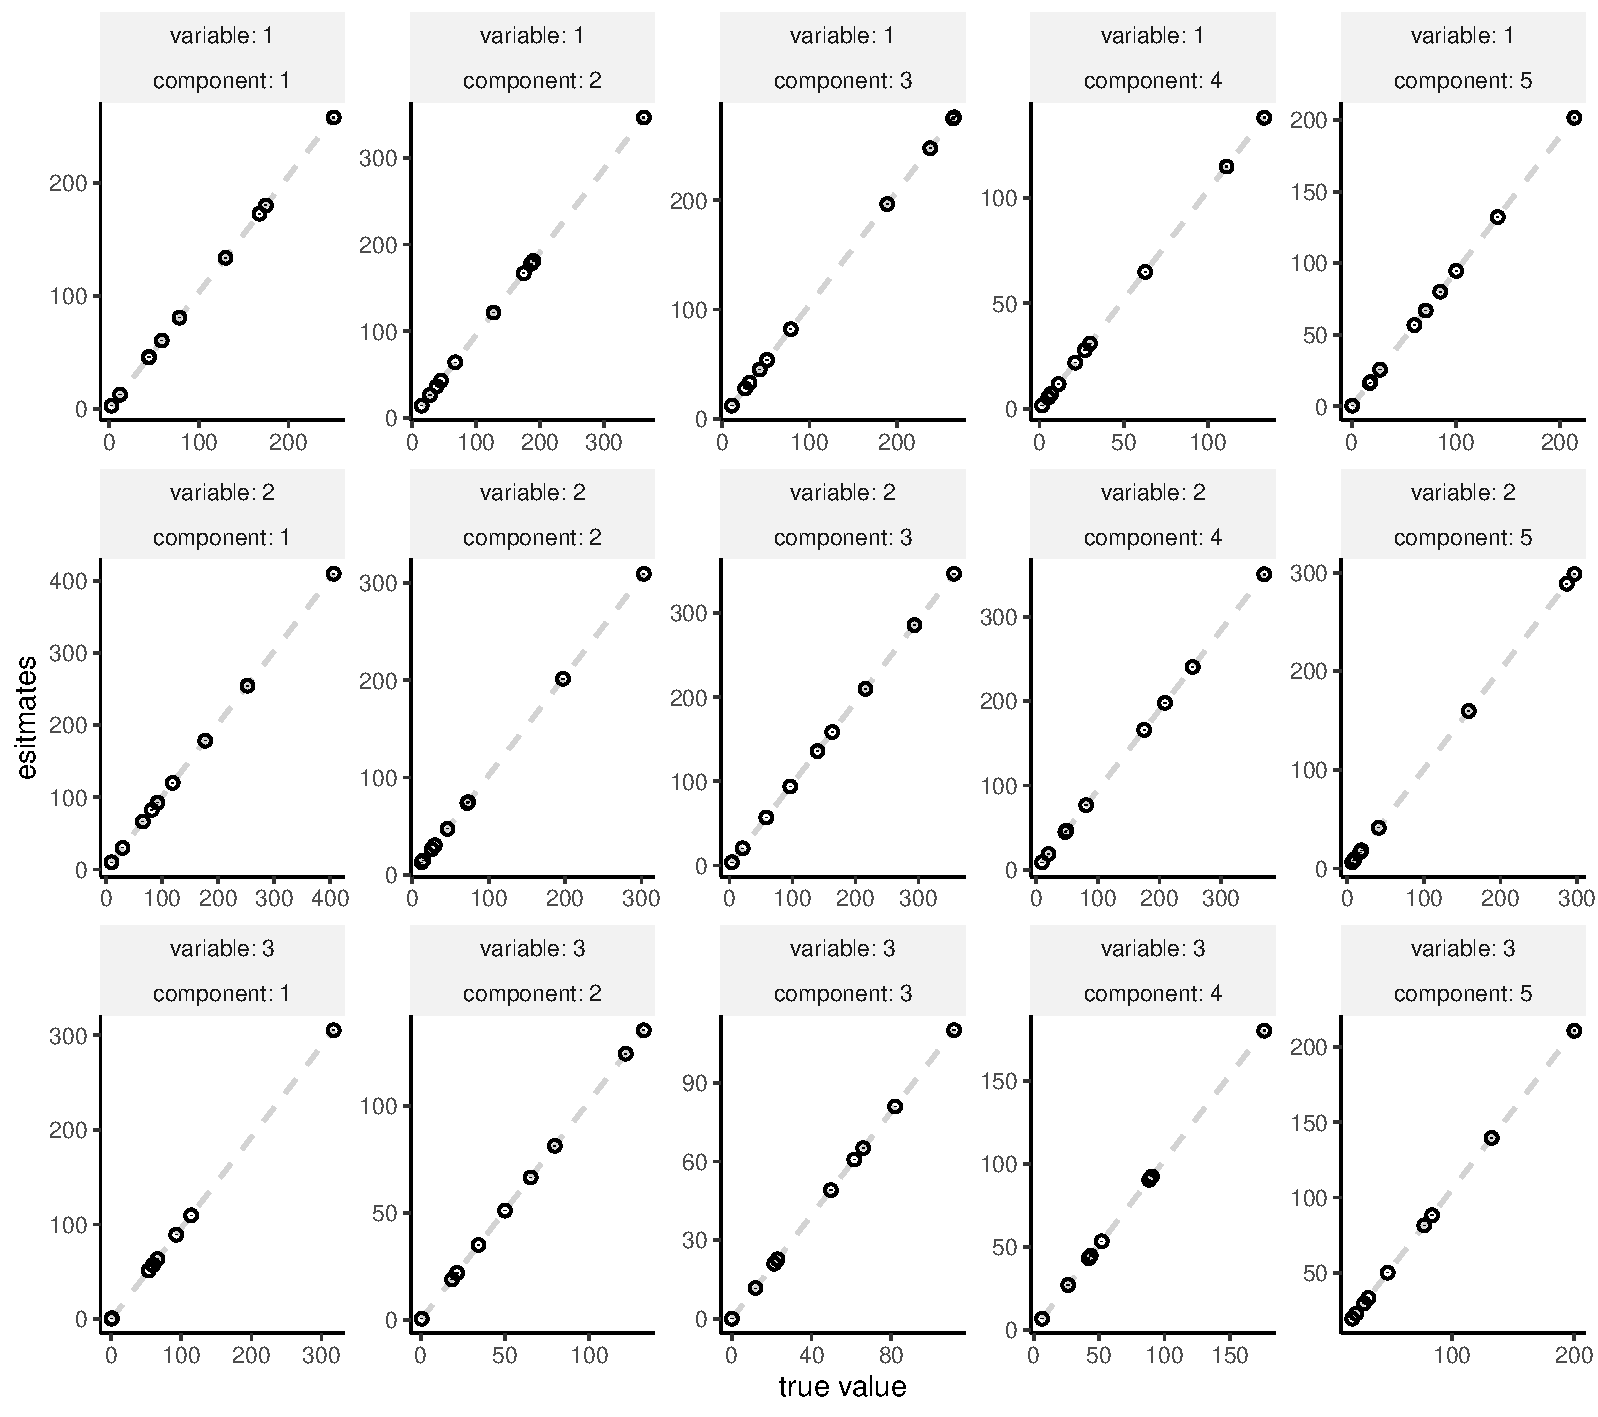
\includegraphics[width=7cm]{img/simV.pdf}
\caption{シミュレーションで設定した真値と 100 回のシミュレーションから得られた推定値の平均の比較. 縦棒: 標準誤差.}
\end{figure}
}
\frame{
\frametitle{モデル選択}
\begin{figure}
\centering
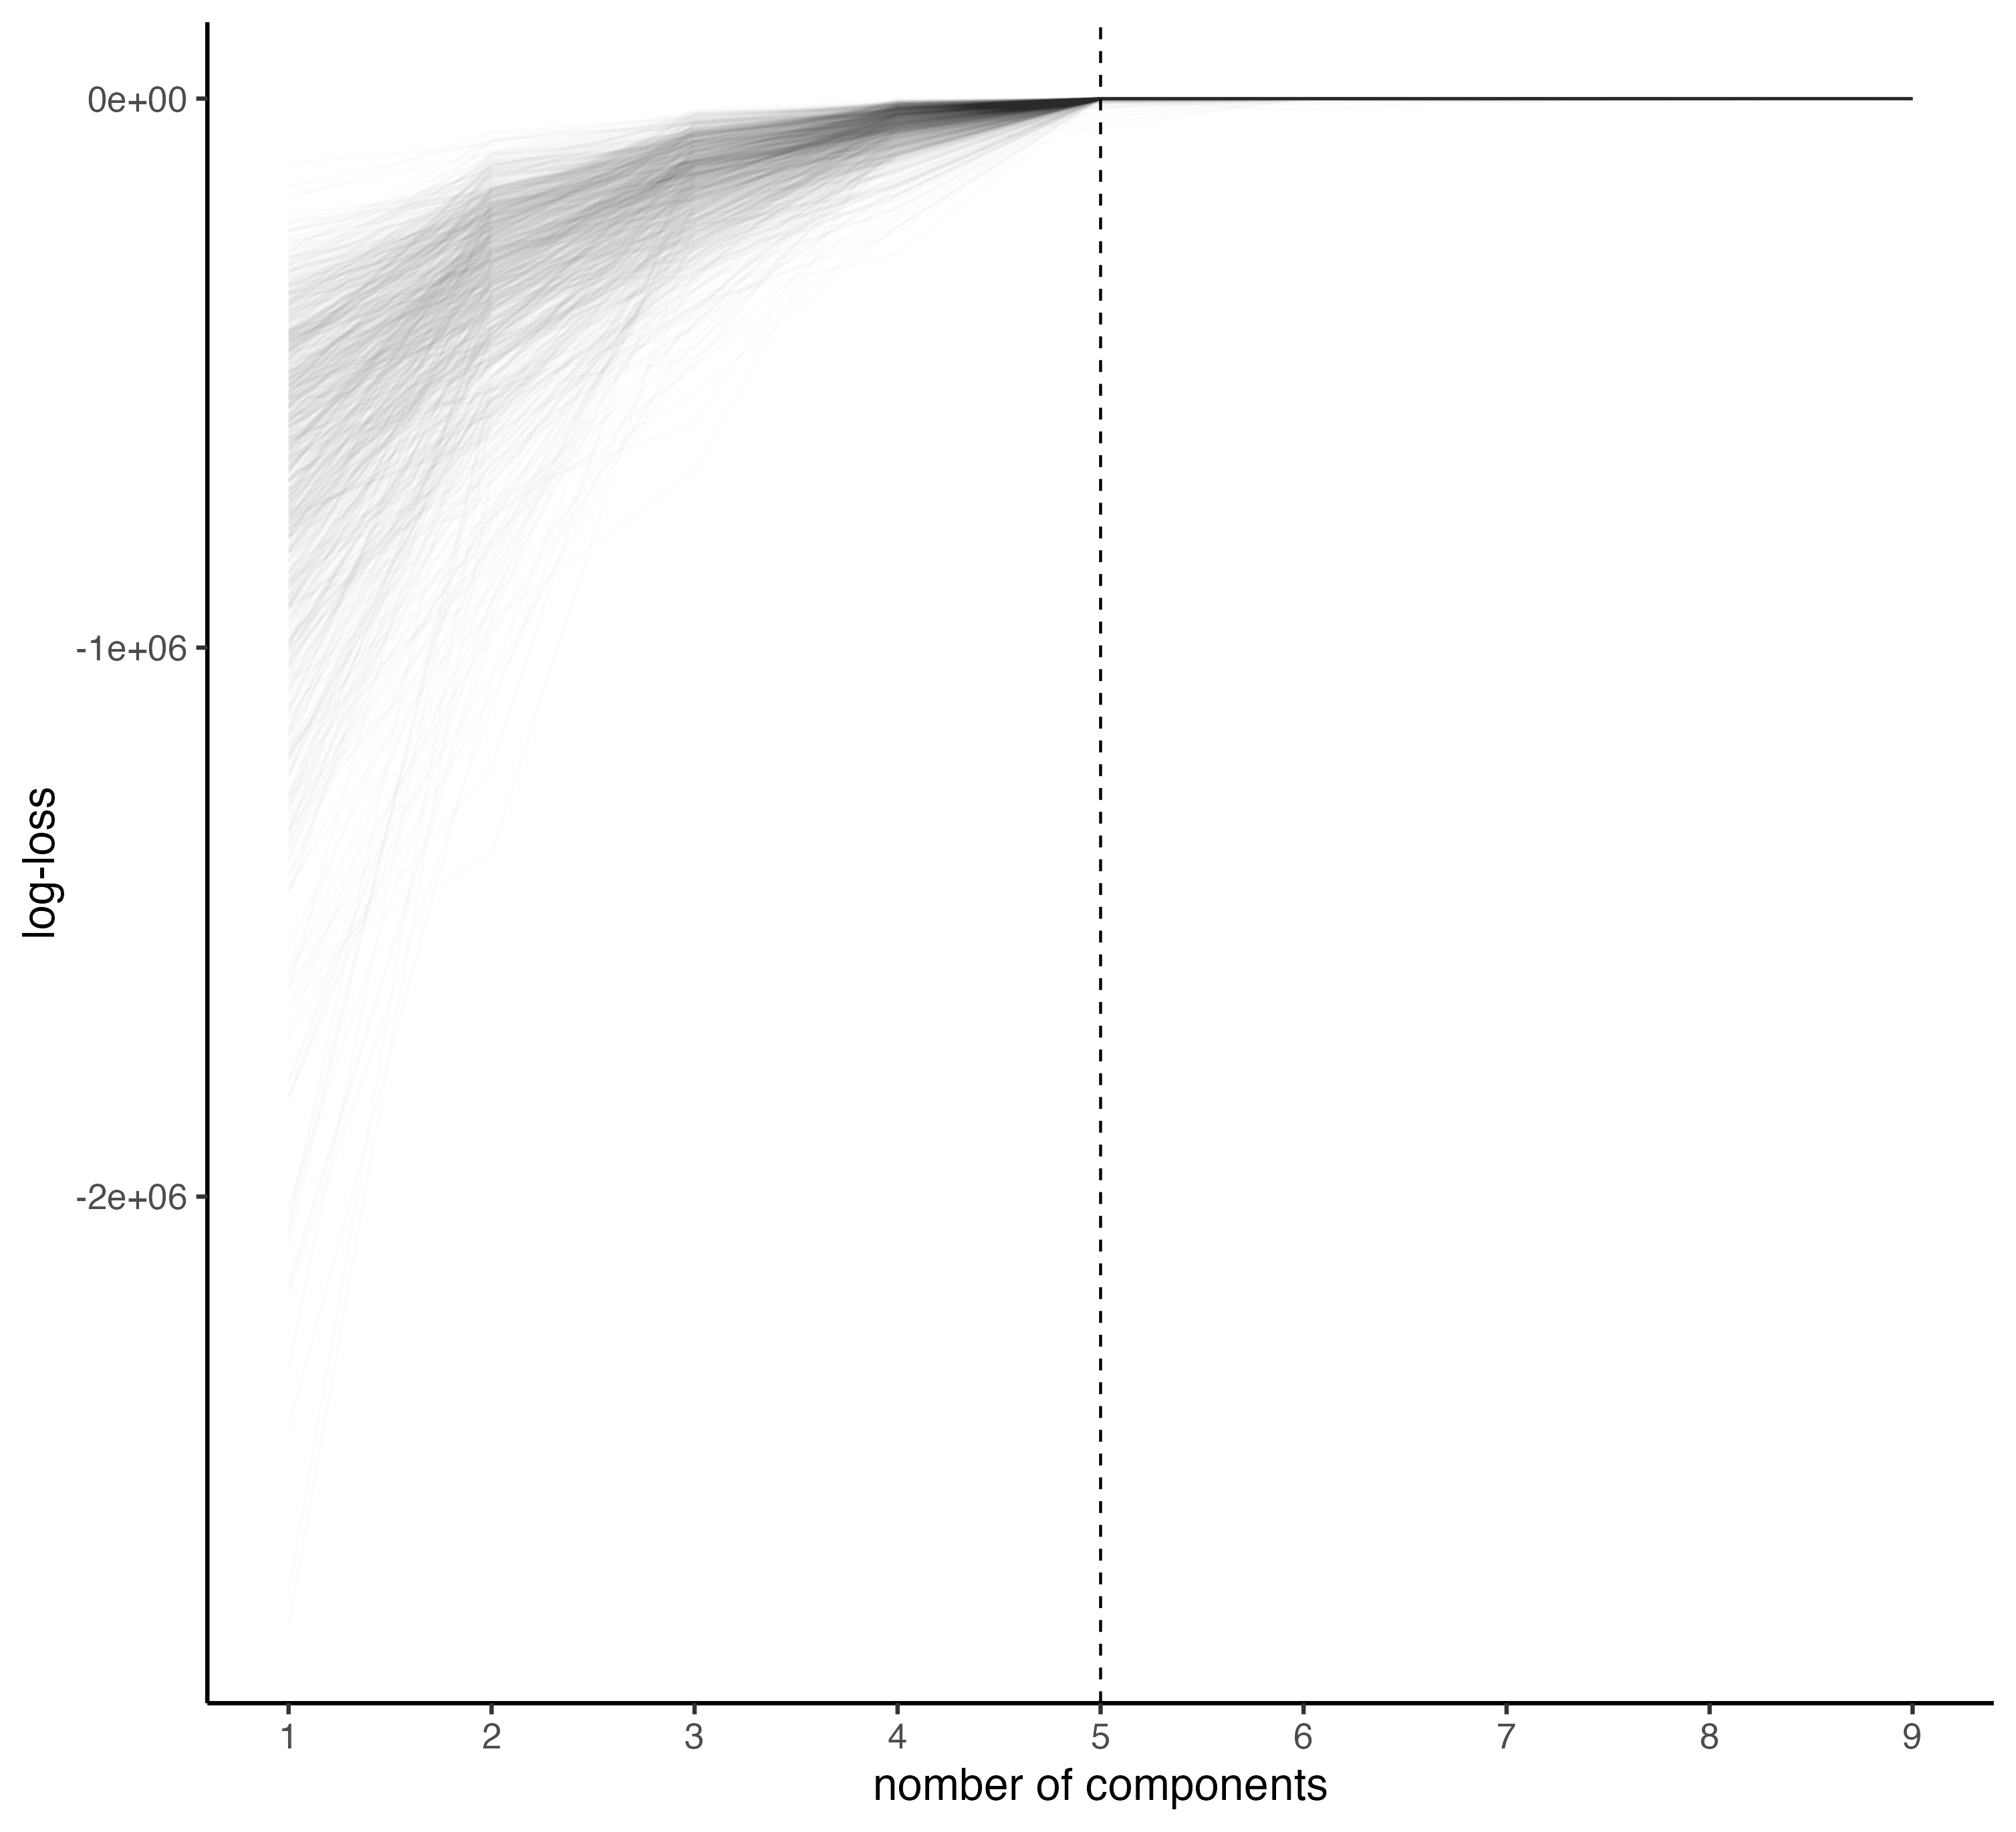
\includegraphics[width=6cm]{img/sim_holdout.png}
\caption{データの10\%をホールドアウトしてテストデータとし, 対数尤度を評価. 1000 回の試行中, $L = 5$ (正解)が 644 回選択}
\end{figure}
}
\section{データ分析}

\begin{frame}[fragile]
\frametitle{簡単な例:予測}

\begin{figure}
\centering
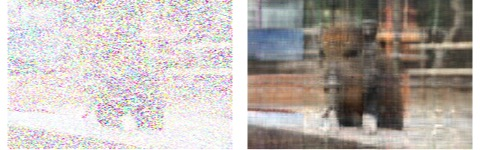
\includegraphics[width=12cm]{img/uri_imp.jpeg}
\caption{左:データとした画像, 右:欠損値を補完した画像. }
\end{figure}
画像の8割をランダムに欠損させ, $L=15$としたUNMFで補完. 左図は欠損値に1を入れて表示. 
\begin{verbatim}
R> mNMF_vb(Y~row+col+rgb, data=X, L=15)
 \end{verbatim}
\end{frame}
%%%
\begin{frame}[fragile]
\frametitle{簡単な例:タイタニックデータ}

\begin{figure}
\centering
\begin{tabular}{cc}
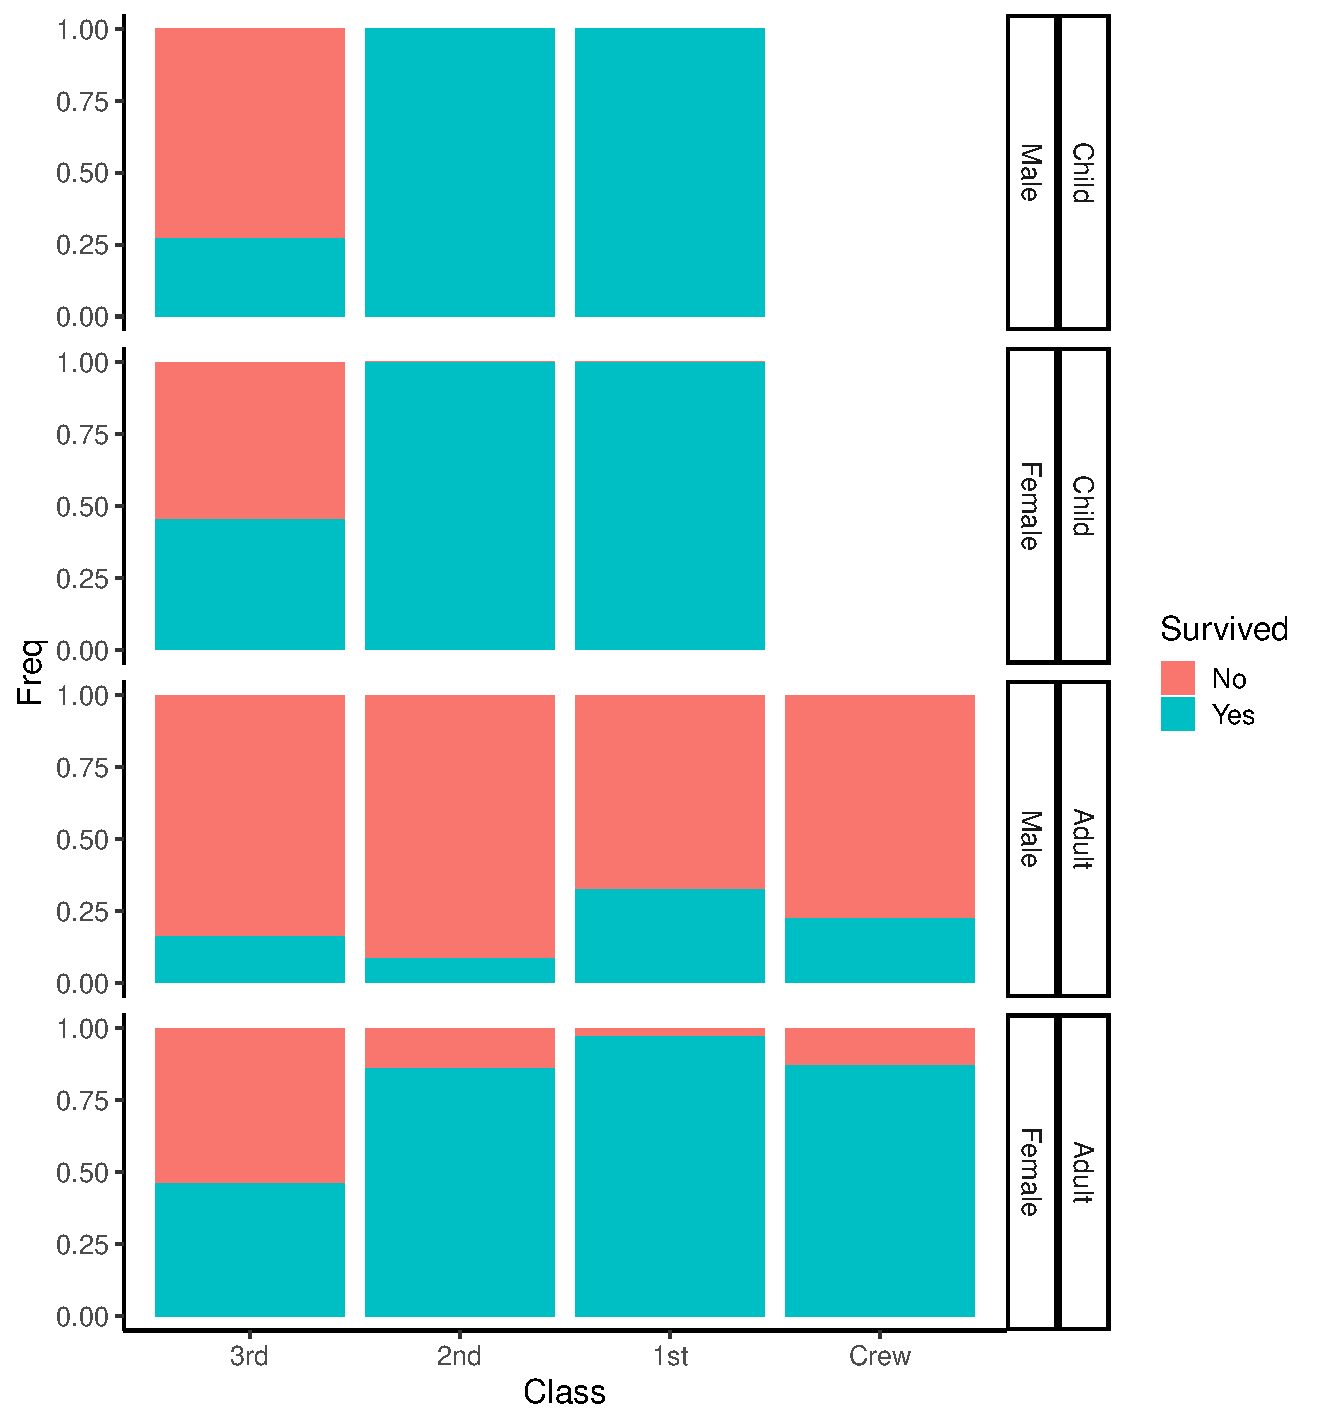
\includegraphics[width=5.5cm]{img/Titanic.pdf} & 
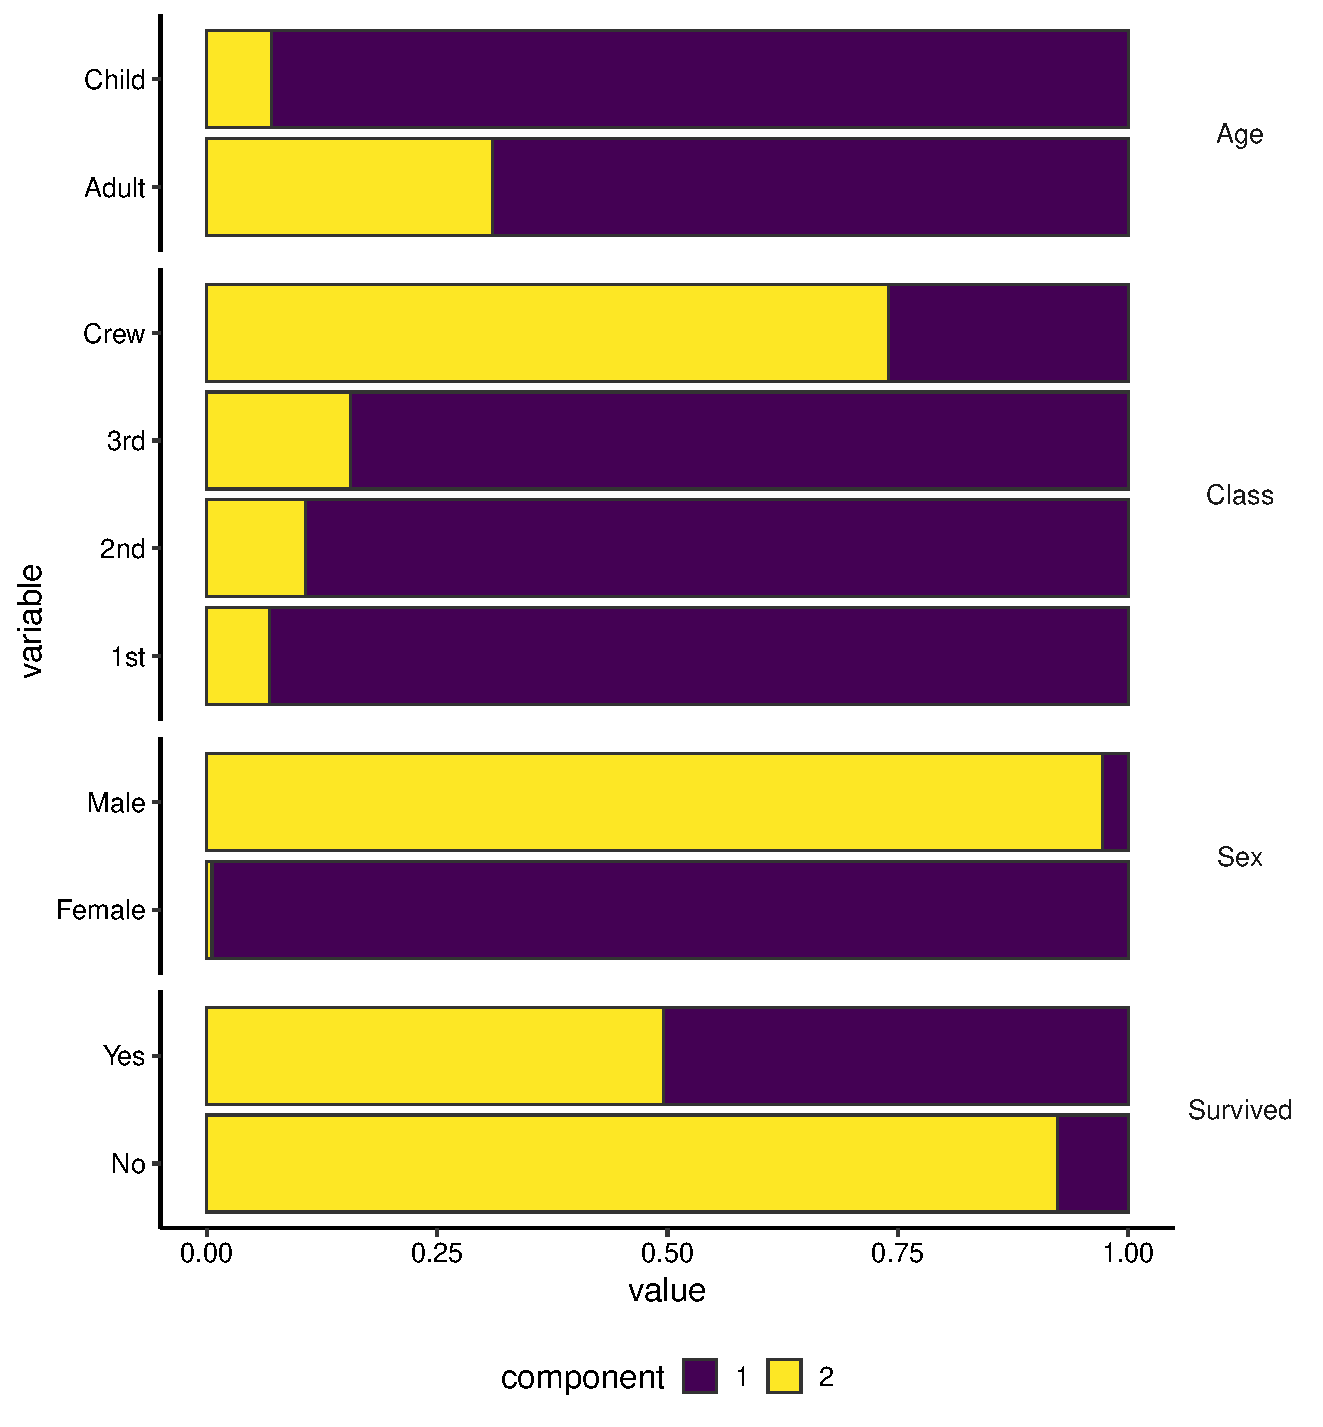
\includegraphics[width=5.5cm]{img/Titanic_V.pdf} 
\end{tabular}
\caption{左:集計されたデータ, 右:$V$の推定値}
\end{figure}

\begin{verbatim}
R> mNMF_vb(Freq ~ Survived+Class+Sex+Age, data=Titanic, L=2)
\end{verbatim}
\end{frame}

\frame{
\frametitle{メタゲノムデータ}

\begin{itemize}
\item David \textit{et al.}(2014) \footnote{David LA, Materna AC, Friedman J, \textit{et al.} (2014). Host lifestyle affects humanmicrobiota on daily timescales. {\em Genome Biology}, 15(R89). \url{https://doi.org/10.1186/gb2014-157-r89}.}は糞便から採取したメタゲノムを縦断的に調査
\item 今回はドナーBについてのみ分析
\item ドナー B については, 530 種の細菌(不明な種は``unknown" としてまとめて集計)が 176 の時点で記録
\item ドナー B は 151日目から159 日目の間に腸管感染症に罹患
\end{itemize}
}
\frame{
\begin{figure}
\centering
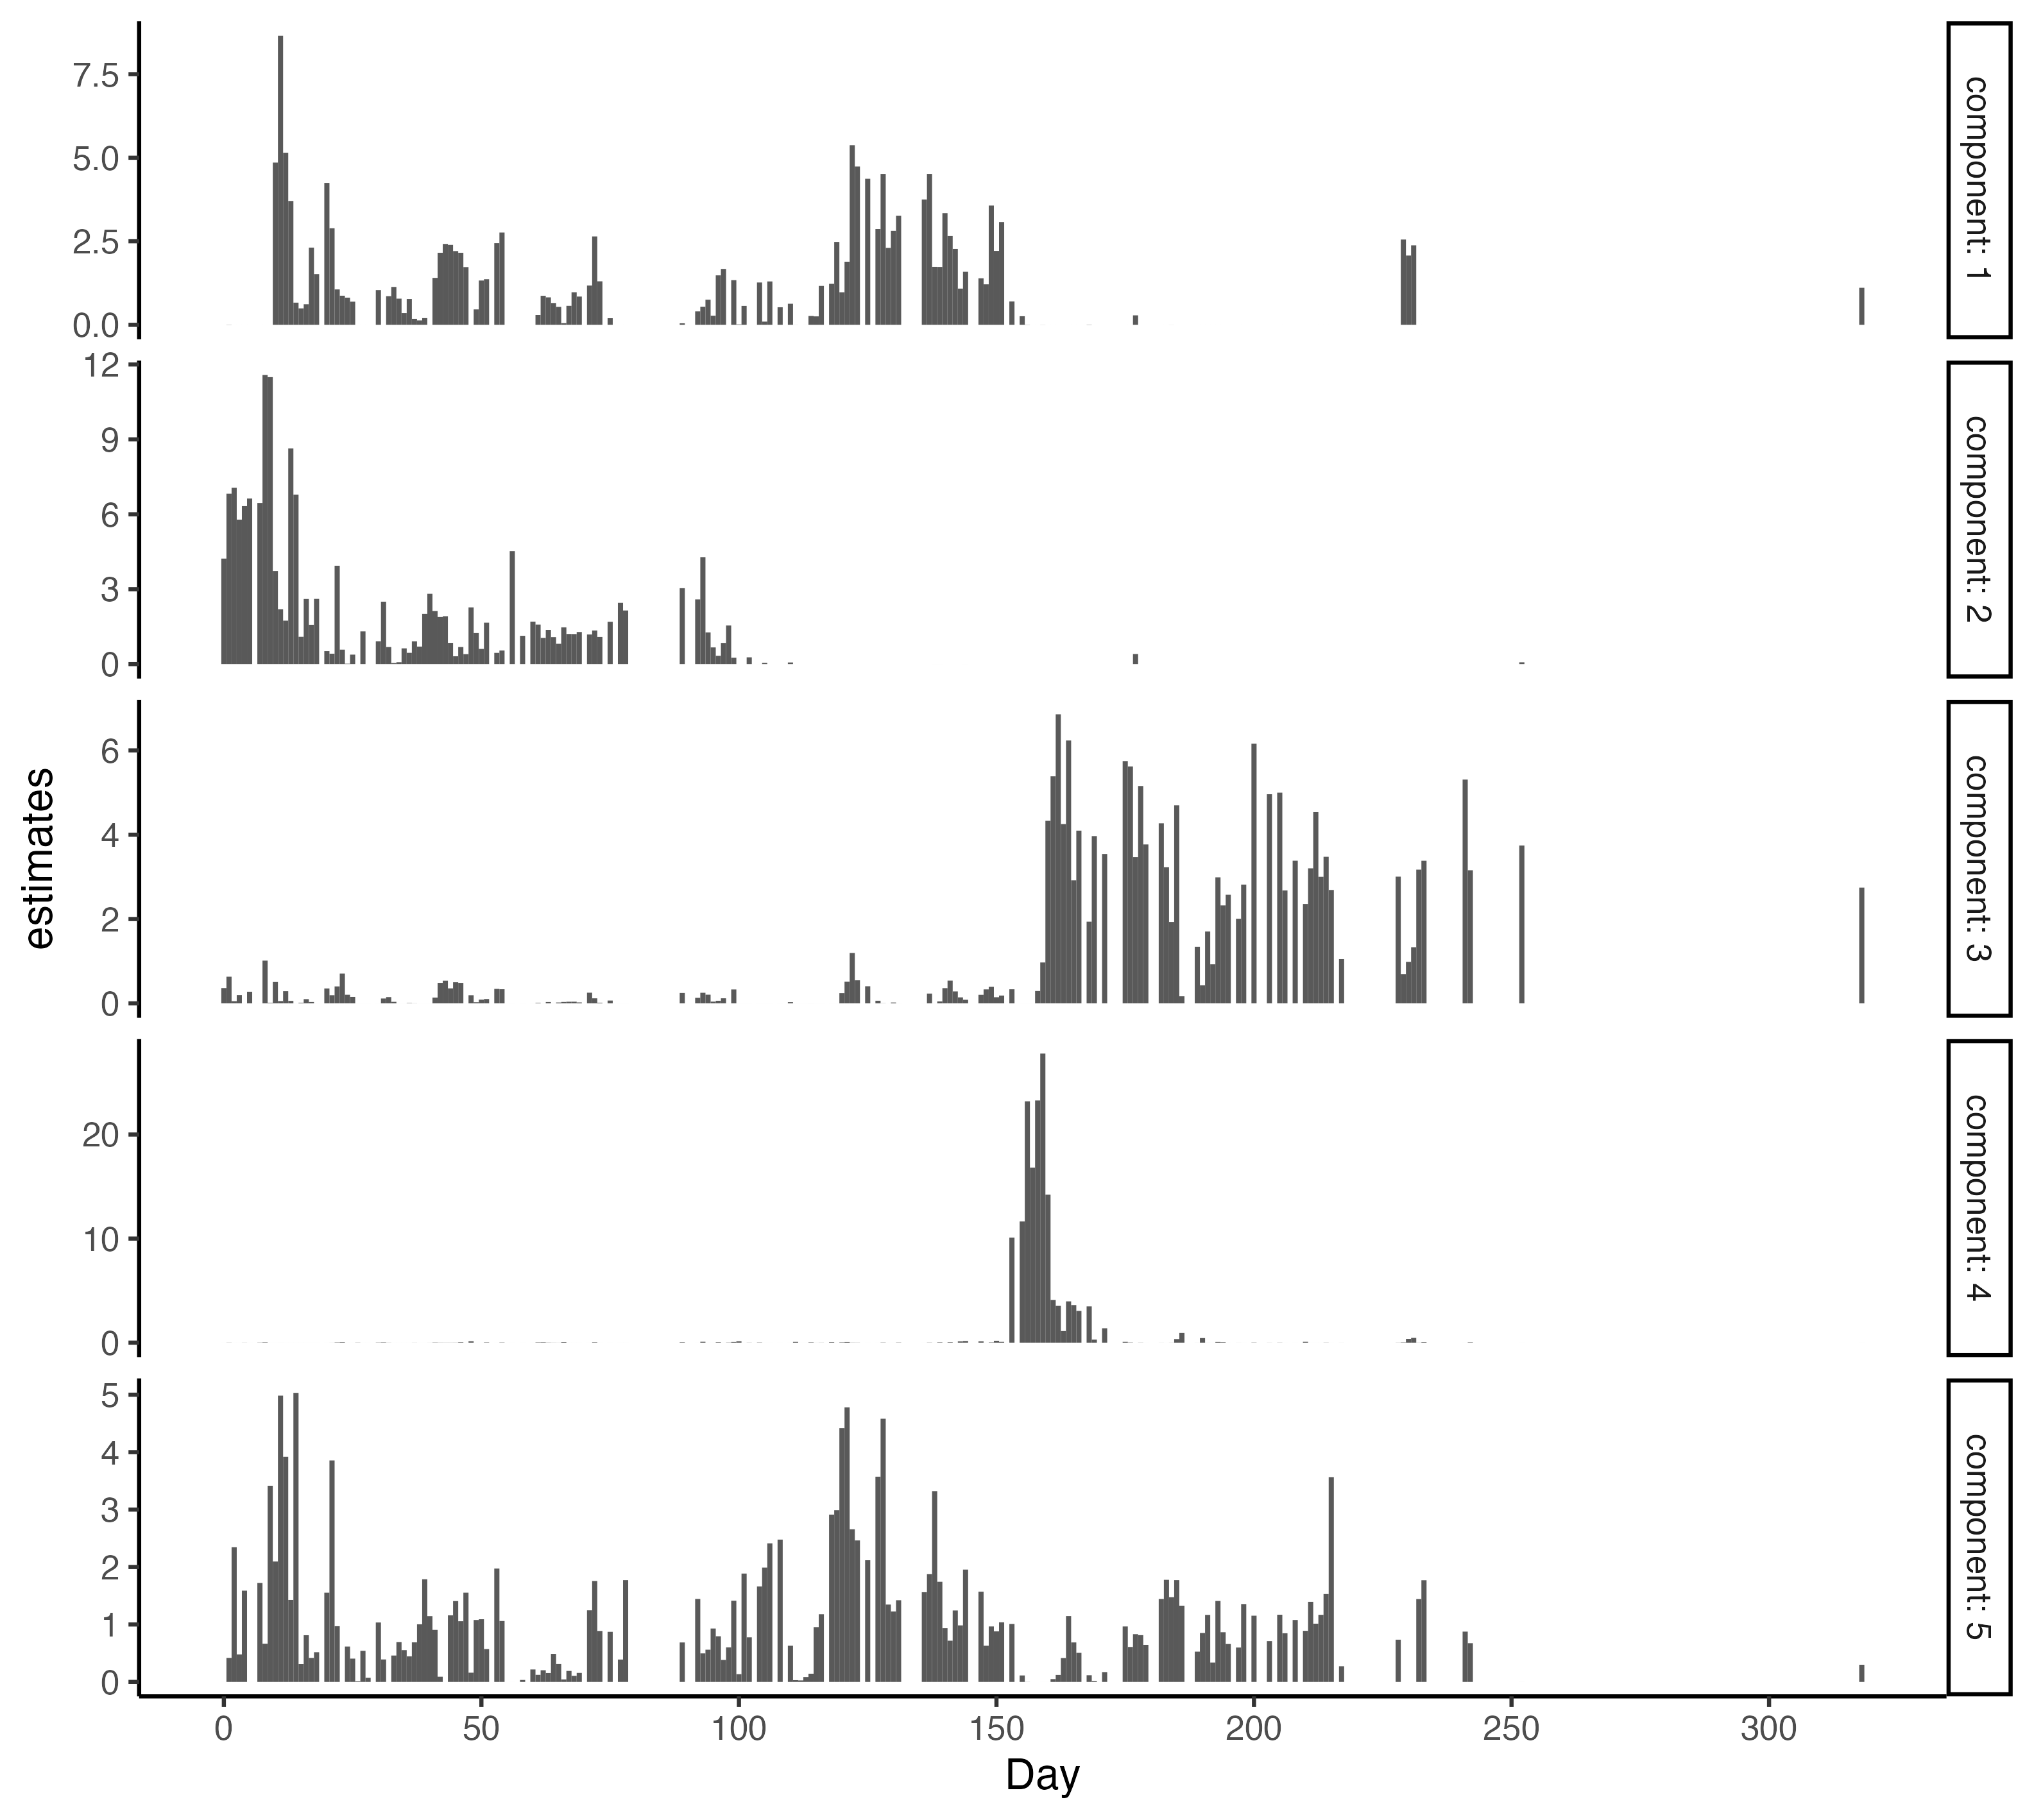
\includegraphics[width=8.5cm]{img/david_day.png} 
\caption{推定された$V$の時間ダミーに対応する部分}
\end{figure}
}
\frame{
\begin{figure}
\centering
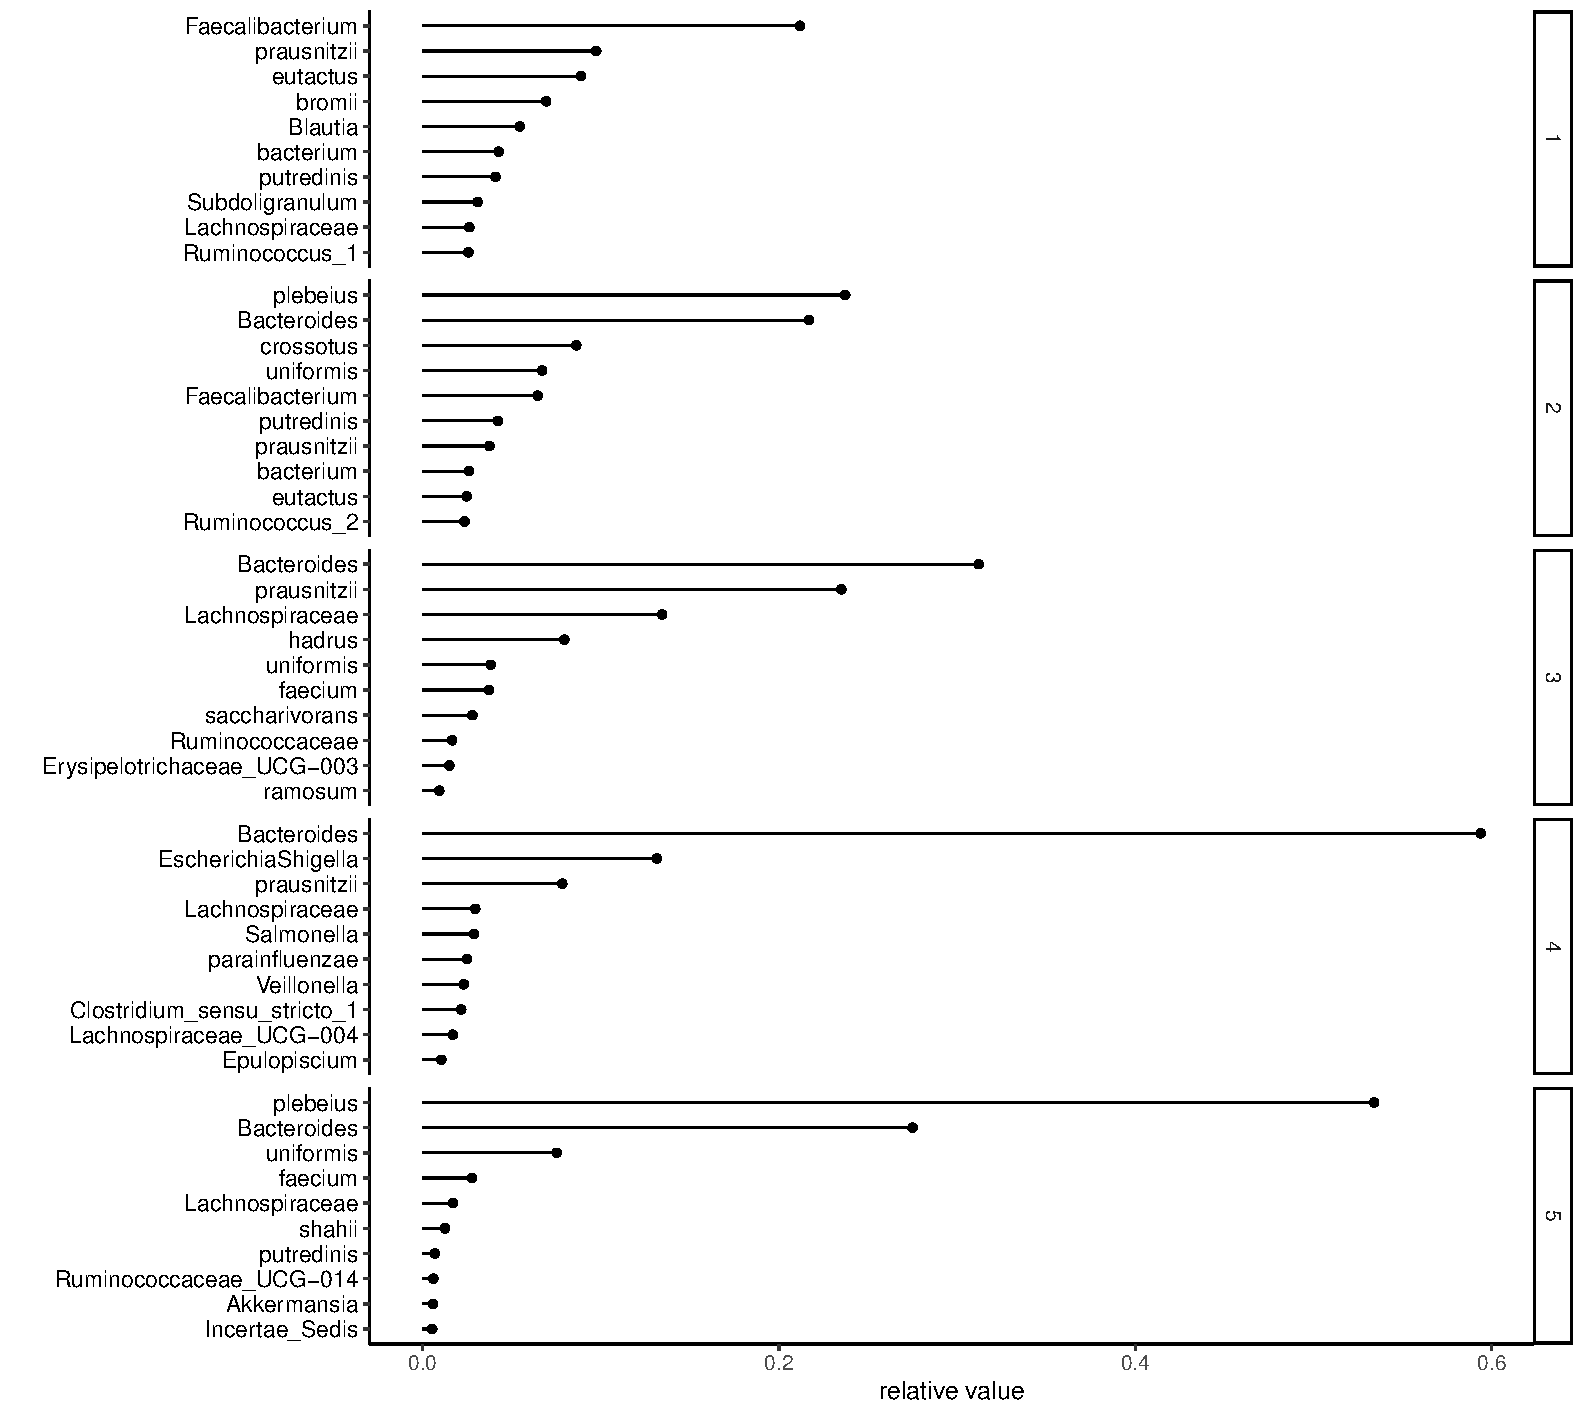
\includegraphics[width=8cm]{img/david_genus.pdf}
\caption{推定された$V$の菌種ダミーに対応する部分. 代表的な細菌上位10種のみ.}
\end{figure}
}
\frame{
\frametitle{遺伝子発現解析}
\begin{itemize}
\item 薬物に対する遺伝子発現応答は創薬の知識につながる
\item 細胞, 遺伝子, 薬剤投与量といった条件の組み合わせは多数になり, 薬剤反応の遺伝子発現データには欠損値が多数存在
\item 薬物反応遺伝子発現データにおける欠損値の補完が求められる
\item 遺伝子発現オムニバス データベース (GEO) から取得した遺伝子発現プロファイル (GSE92742) を分析
\item 遺伝子$\times$時間$\times$細胞タイプ$\times$投与量
\item 補完の精度を評価するために, データのレコードをランダムに削除し, 学習用に
\end{itemize}
}
\frame{
\frametitle{予測の比較}
\begin{table}[htb]
\caption{RMSEの比較. GSE データを $10^6$ 行にリサンプリングし, $10^5$ をテスト データとして、残りを検証用とした}
\centering
\begin{tabular}{r}
\begin{tabular}{rrrr|r}
  \hline
\multicolumn{4}{c|}{hyperparameter} & (XGBoost)\\
 eta & max\_depth & lambda & alpha & RMSE \\ 
  \hline
 0.30 & 6.00 & 1.00 & 0.00 & 1314.17 \\ 
 0.30 & 5.00 & 0.50 & 0.00 & 1340.58 \\ 
0.50 & 15.00 & 0.50 & 0.10 & 1032.77 \\ 
1.50 & 30.00 & 1.00 & 0.00 & 800.95 \\ 
\hline
& & & & (UNMF)\\
& & & L & RMSE \\ 
\hline
& & & 2 & 816.67 \\ 
& & & 3 & 780.11 \\ 
& & & 4 & 762.93 \\ 
& & & 5 & 763.50 \\ 
\hline
\end{tabular}
\end{tabular}
\end{table}
}
\frame{
\frametitle{予測の比較(デフォルト)}
\begin{figure}
\centering
\begin{tabular}{cc}
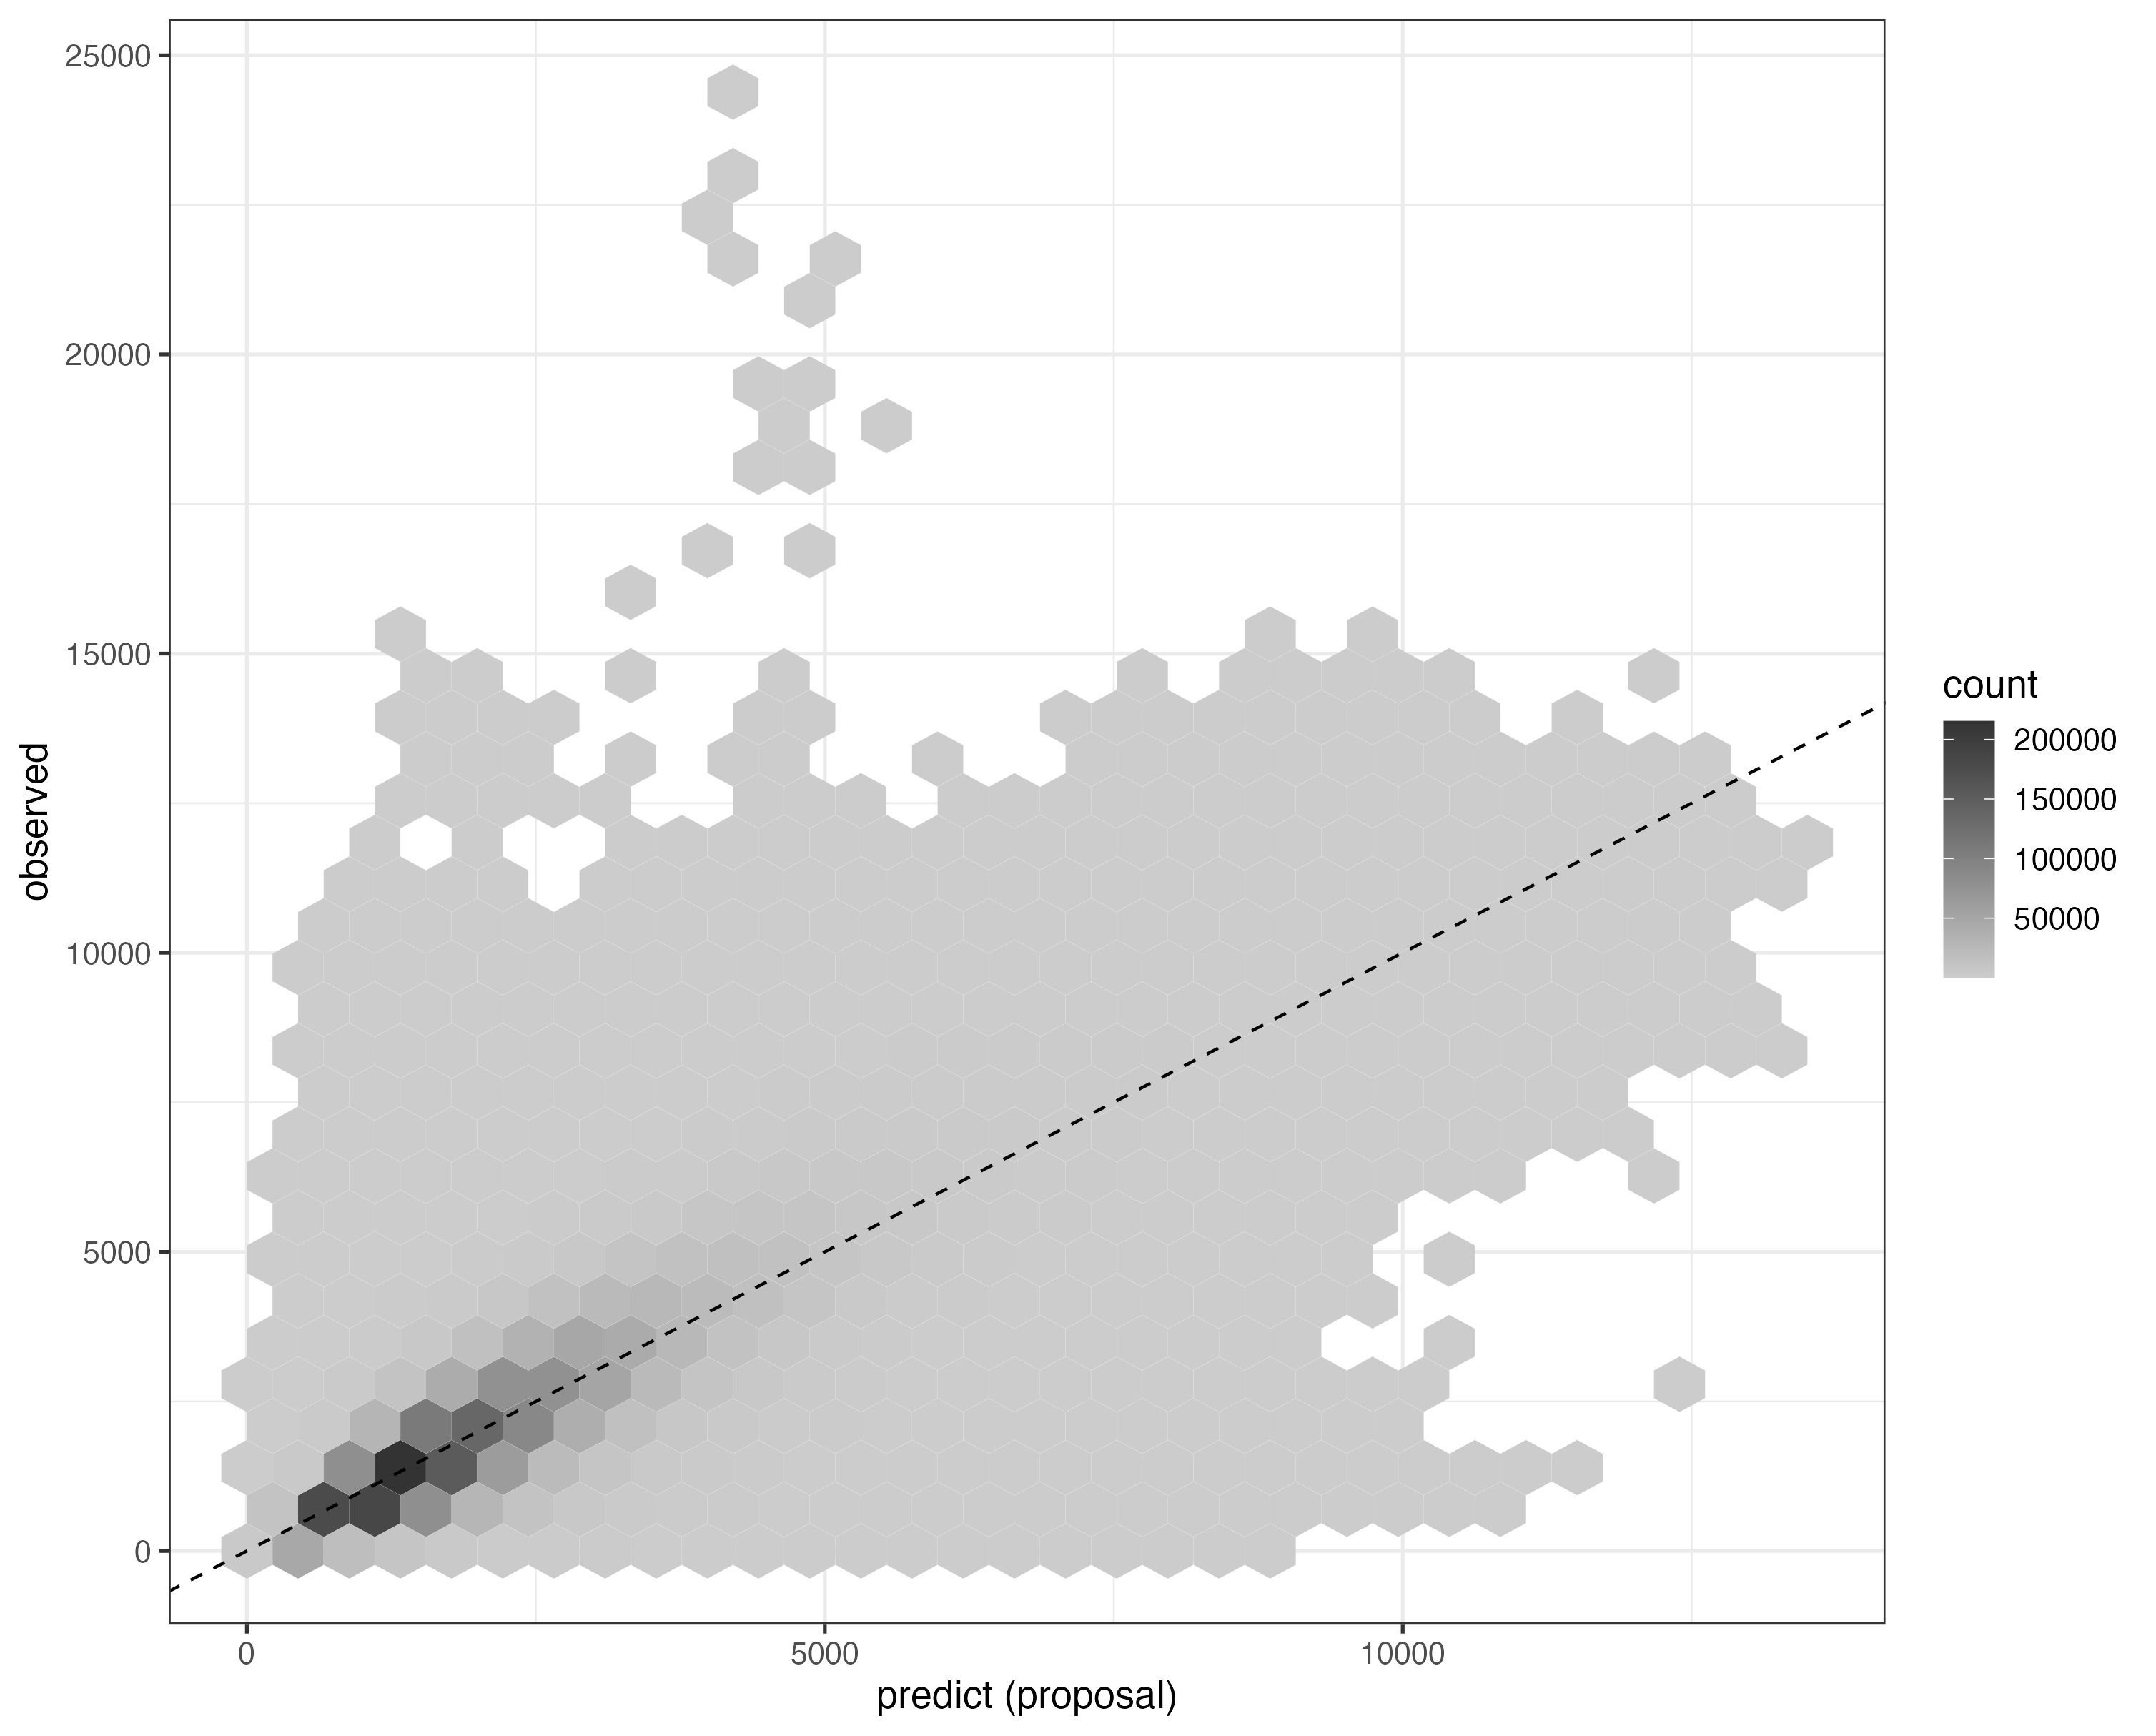
\includegraphics[width=5cm, clip]{./img/gse_pred.png} &
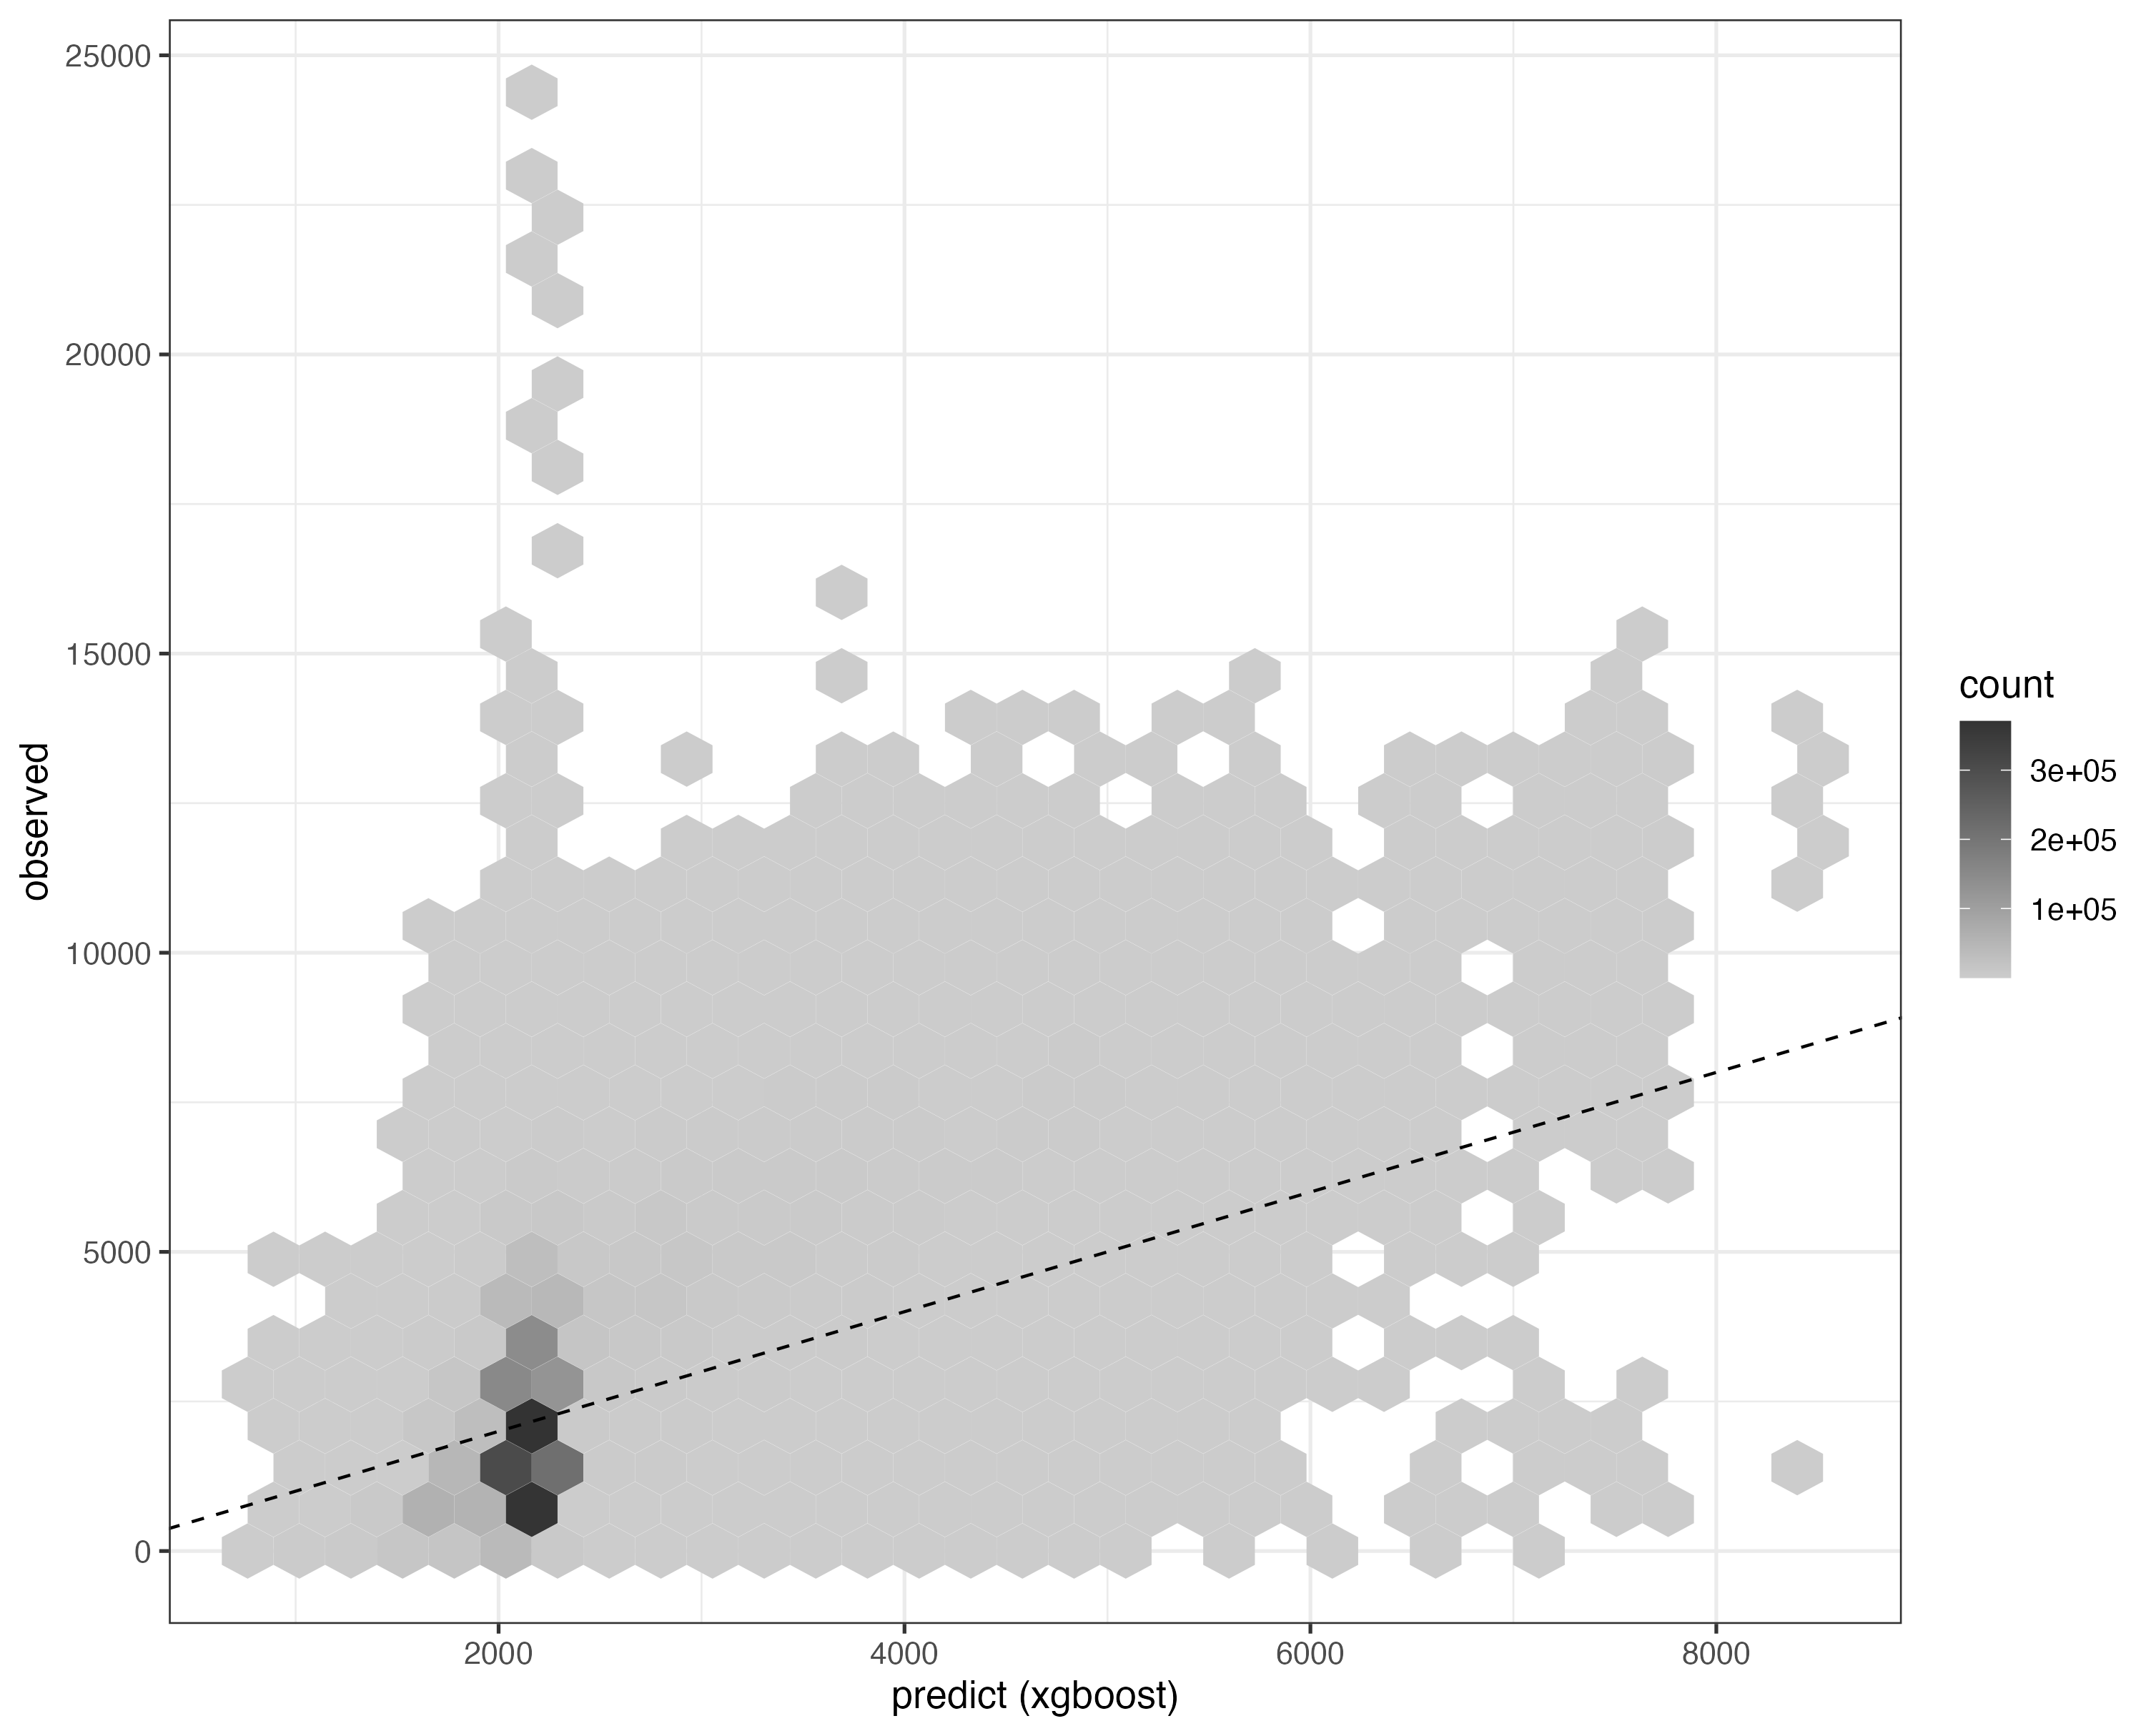
\includegraphics[width=5cm, clip]{./img/gse_pred_xgboost.png}
\end{tabular}
\caption{x軸: 予測, y軸: 実測値 (正解). 左: UNMF, 右: xgboost}
\label{figGSE}
\end{figure}
}
\frame{
\frametitle{まとめ}
 \begin{itemize}
\item UNMF は欠測値や反復測定を含む幅広いデータ形式を扱える
\item 解釈性を維持したまま予測精度を実現
\item 「前処理」が正規化, 平滑化, 欠測値の補完といった複数のステップからなる場合, 分析全体としての自由度は多重に大きくなり, 検証はより複雑になる
\item そのため一つのモデルで予測と解釈, 検証を行えることは重要
\item  今後の研究:マルチタスク・マルチモーダル学習
\end{itemize}
}
\end{document}  